\section{Aproximação de curta distância}
\label{sec:cap4_app_curta}

Nesta seção são apresentados os resultados da aproximação de curta distância no referencial \gls{lvlh}{,} com ênfase na evolução da posição relativa{,} da velocidade relativa e das acelerações de controle aplicadas ao perseguidor. As grandezas numéricas foram obtidas diretamente a partir dos sinais exportados do modelo em ambiente Simulink.

A Tabela~\ref{tab:cap4_app_curta_condicoes_lvhl} apresenta as condições iniciais e as medições finais da aproximação de curta distância em \gls{lvlh}{,} expressas pelas componentes along-track{,} cross-track e radial. Em complemento{,} a Figura~\ref{fig:cap4_posicoes_lvlh} apresenta{,} de forma gráfica{,} a evolução dessas componentes ao longo do tempo. Esses valores iniciais decorrem da conversão{,} para o referencial \gls{lvlh}{,} dos vetores de posição em ECI no instante final da aproximação de longa distância.

\begin{table}[H]
\centering
\caption{Condições iniciais e medições finais da aproximação curta (LVLH).}
\label{tab:cap4_app_curta_condicoes_lvhl}
\begin{tabularx}{\linewidth}{|
  >{\raggedright\arraybackslash}X|
  >{\raggedleft\arraybackslash}X|
  >{\raggedleft\arraybackslash}X|
  >{\centering\arraybackslash}X|}
\hline
\multicolumn{1}{|c|}{\textbf{Grandeza}} &
\multicolumn{1}{c|}{\textbf{Medição inicial}} &
\multicolumn{1}{c|}{\textbf{Medição final}} &
\multicolumn{1}{c|}{\textbf{Unidade}} \\
\hhline{|=|=|=|=|}
Posição along-track          & $-353{,}777$ & $-0{,}007$   & m \\
\hline
Posição radial               & $-100{,}009$ & $-0{,}500$   & m \\
\hline
Posição cross-track          & $0{,}000$    & $0{,}000$    & m \\
% Norma da posição relativa    & $367{,}641$  & $0{,}500$    & m \\
% Norma da posição relativa    & $0{,}367641$ & $0{,}000500$ & km \\
\hline
\end{tabularx}
\end{table}
 
\begin{figure}[H]
\centering

\includegraphics[width=1\linewidth]{4 Resultados e discussoes/Imagens/2 App curta distancia/1 Posicao e distancia relativa (LVLH).png}
\caption{Posições do perseguidor no referencial \gls{lvlh}.}
    \label{fig:cap4_posicoes_lvlh}
\end{figure}

A Figura~\ref{fig:cap4_posicoes_lvlh} mostra a evolução temporal das componentes de posição relativa entre o perseguidor e o alvo no referencial \gls{lvlh} durante a aproximação de curta distância. 
Próximo ao final do intervalo de simulação foram inseridas duas linhas verticais que indicam os instantes de assentamento das componentes radial e along-track.

O critério de assentamento (estabilização) adotado consiste em permanecer dentro de uma faixa de tolerância de $\pm 0{,}05$ m em torno dos valores finais da Tabela~\ref{tab:cap4_app_curta_condicoes_lvhl}{,} durante pelo menos $15$ s.
Com esse critério{,} a componente radial atinge o regime permanente em aproximadamente $515$ s{,} enquanto a componente along-track se estabiliza em torno de $530$ s; a componente cross-track permanece dentro da banda de tolerância desde o início da aproximação de curta distância.

% Ademais{,} as Figuras~\ref{fig:cap4_proj_3d} e~\ref{fig:cap4_projecao} apresentam as projeções do deslocamento relativo do perseguidor em relação ao alvo durante a fase de translação.

\begin{figure}[H]
\centering
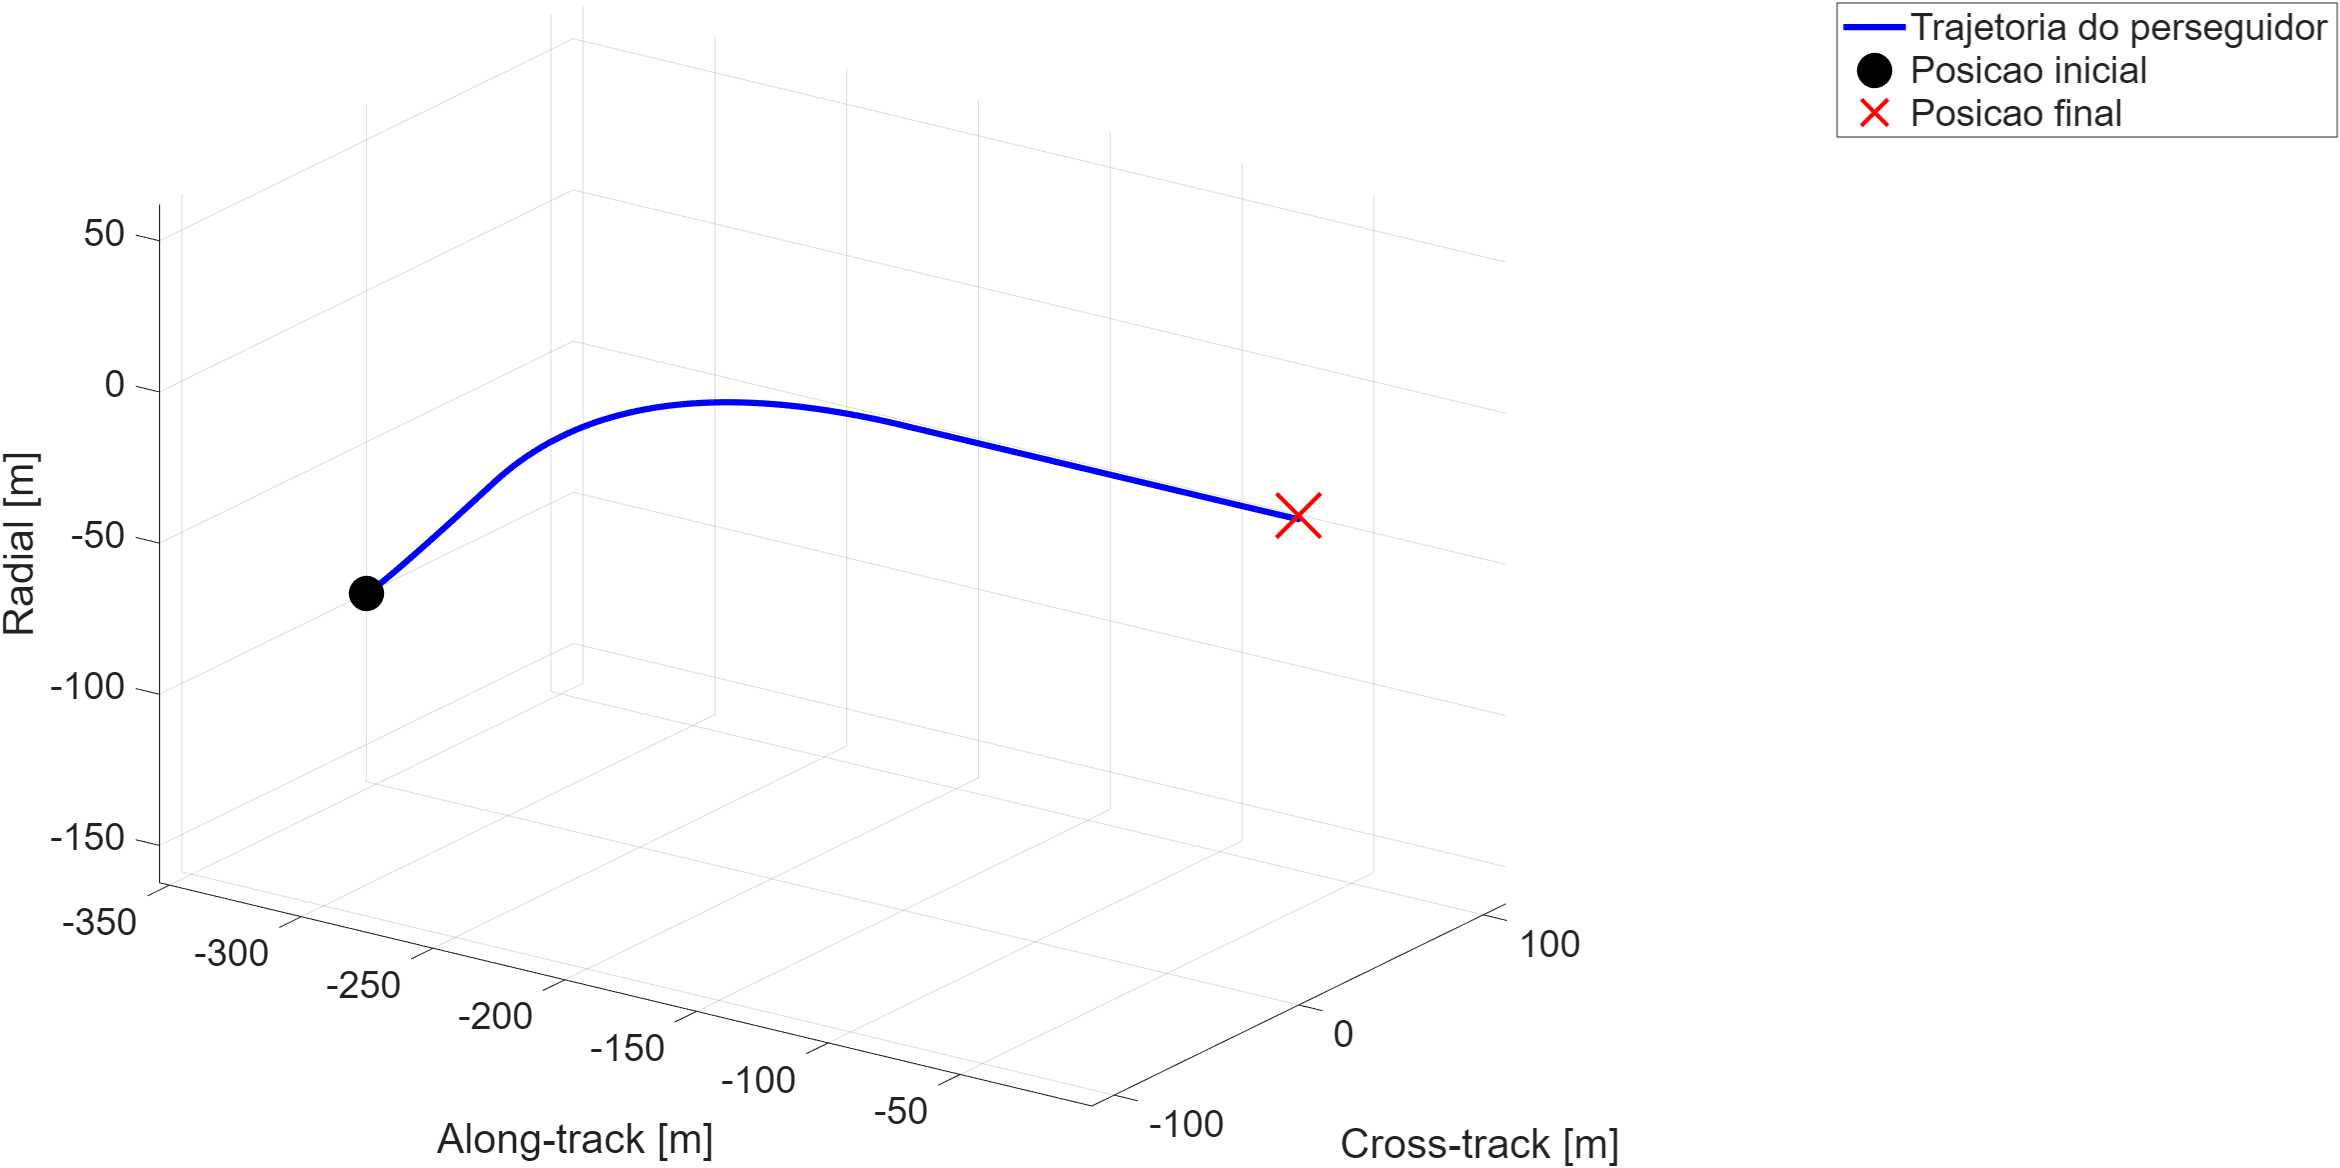
\includegraphics[width=1\linewidth]{4 Resultados e discussoes/Imagens/2 App curta distancia/4 Projecao 3D.png}
\caption{Projeção tridimensional do deslocamento perseguidor em relação ao alvo no referencial \gls{lvlh}.}
    \label{fig:cap4_proj_3d}
\end{figure}

A Figura~\ref{fig:cap4_proj_3d} apresenta o deslocamento do perseguidor em uma visão tridimensional{,} enquanto a Figura~\ref{fig:cap4_projecao} exibe a mesma trajetória em projeções bidimensionais{,} combinando os pares de eixos radial–along-track{,} cross-track--along-track e cross-track--radial.

\begin{figure}[H]
\centering
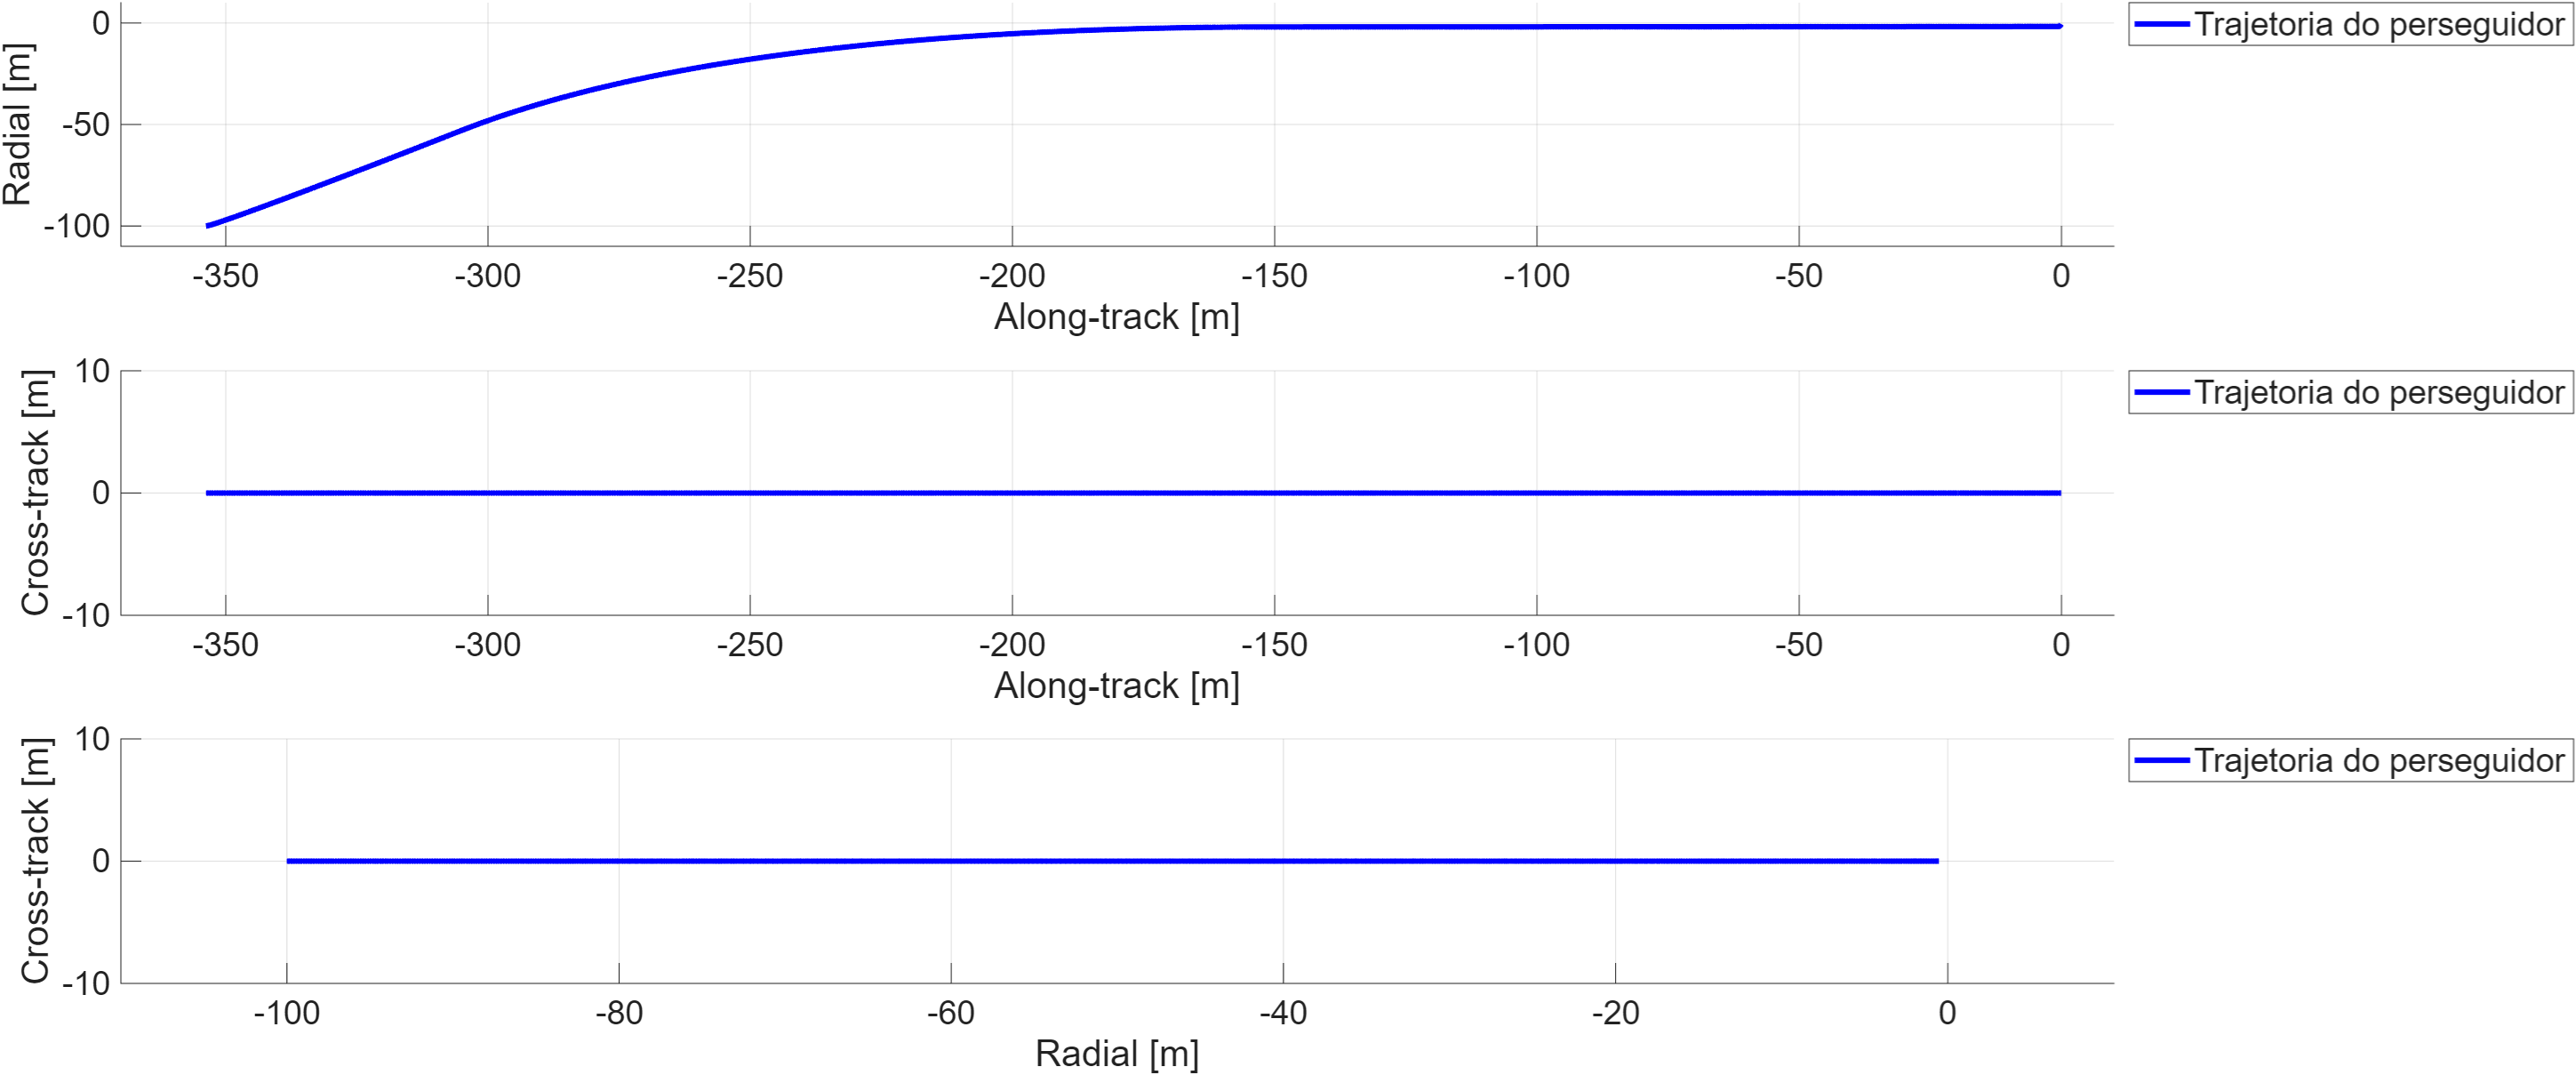
\includegraphics[width=1\linewidth]{4 Resultados e discussoes/Imagens/2 App curta distancia/5 Projecao along radial e cross.png}
\caption{Projeções do deslocamento perseguidor em relação ao alvo no referencial \gls{lvlh}.}    \label{fig:cap4_projecao}
\end{figure}

\subsection{Velocidade relativa}

O comportamento da velocidade relativa no referencial \gls{lvlh} é sintetizado na Tabela~\ref{tab:cap4_app_curta_vel_lvhl}{,} que reúne os valores inicial e final de cada componente{,} bem como a norma da velocidade relativa ao longo da aproximação de curta distância.

\begin{table}[H]
\centering
\caption{Velocidade relativa inicial e final em LVLH e norma correspondente.}
\label{tab:cap4_app_curta_vel_lvhl}
\begin{tabularx}{\linewidth}{|
  >{\raggedright\arraybackslash}X|
  >{\raggedleft\arraybackslash}X|
  >{\raggedleft\arraybackslash}X|
  >{\centering\arraybackslash}X|}
\hline
\multicolumn{1}{|c|}{\textbf{Grandeza}} &
\multicolumn{1}{c|}{\textbf{Valor inicial}} &
\multicolumn{1}{c|}{\textbf{Valor final}} &
\multicolumn{1}{c|}{\textbf{Unidade}} \\
\hhline{|=|=|=|=|}
Velocidade along-track & $0{,}162462$ & $0{,}000012$ & m/s \\
\hline
Velocidade cross-track & $0{,}000000$ & $0{,}000000$ & m/s \\
\hline
Velocidade radial & $0{,}000008$ & $0{,}000000$ & m/s \\
\hline
Norma da velocidade relativa & $0{,}162462$ & $0{,}000012$ & m/s \\
% \hline
% Norma da velocidade relativa (máxima) & -- & $0{,}424264$ & m/s \\
\hline
\end{tabularx}
\end{table}

\begin{figure}[H]
\centering

\includegraphics[width=1\linewidth]{4 Resultados e discussoes/Imagens/2 App curta distancia/2 Velocidades relativas (LVLH).png}
\caption{Velocidades do perseguidor no referencial \gls{lvlh}.}
    \label{fig:cap4_velocidades_lvlh}
\end{figure}

A Figura~\ref{fig:cap4_velocidades_lvlh} apresenta a evolução temporal das componentes de velocidade relativa no referencial \gls{lvlh}{,} juntamente com as faixas de limite adotadas para a missão. Estabeleceu-se que{,} para distâncias relativas superiores a $20$ m{,} a velocidade relativa máxima admissível é de $0{,}300$ m/s{,} enquanto para distâncias inferiores a $20$ m o limite é reduzido para $0{,}030$ m/s{,} em conformidade proposto por \cite{vedant2025longrange{,}mathworks_space_rendezvous_docking}.

Observa-se que o sistema de navegação e guiagem mantém o perseguidor dentro desses limites ao longo de toda a aproximação de curta distância. As linhas verticais indicam{,} adicionalmente{,} os instantes em que as componentes radial e along-track passam a satisfazer o critério de assentamento definido na Seção~\ref{sec:cap4_app_curta}{,} isto é{,} permanência dentro da faixa de $\pm 0{,}05$ m em torno dos valores finais por um intervalo mínimo de $15$ s.

\subsection{Tempos de assentamento em posição}

Os tempos de assentamento em cada componente do referencial \gls{lvlh} foram obtidos por meio de um bloco específico de medição no modelo{,} utilizando o mesmo critério de tolerância previamente definido para a estabilização em posição. A Tabela~\ref{tab:cap4_app_curta_tempos_assentamento} resume esses resultados{,} apresentados tanto em segundos quanto no formato horas{,} minutos e segundos.

\begin{table}[H]
\centering
\caption{Tempos de assentamento da aproximação curta em LVLH.}
\label{tab:cap4_app_curta_tempos_assentamento}
\begin{tabularx}{\linewidth}{|
  >{\raggedright\arraybackslash}X|
  >{\raggedleft\arraybackslash}X|
  >{\centering\arraybackslash}X|}
\hline
\multicolumn{1}{|c|}{\textbf{Componente}} &
\multicolumn{1}{c|}{\textbf{Tempo [s]}} &
\multicolumn{1}{c|}{\textbf{Tempo [h]}} \\
\hhline{|=|=|=|}
Radial      & $515{,}200$ & $00\mathrm{h}:08\mathrm{m}:35\mathrm{s}$ \\
Along-track & $530{,}260$ & $00\mathrm{h}:08\mathrm{m}:50\mathrm{s}$ \\
Cross-track & $0{,}000$   & $00\mathrm{h}:00\mathrm{m}:00\mathrm{s}$ \\
\hline
\end{tabularx}
\end{table}

A Figura~\ref{fig:cap4_erro_radial} apresenta o erro de posição no eixo radial ao longo do tempo no referencial \gls{lvlh}. As linhas tracejadas indicam a faixa de tolerância em torno do valor final desejado{,} enquanto a linha vertical vermelha marca o instante em que o erro passa a permanecer dentro dessa faixa pelo intervalo mínimo de tempo adotado{,} caracterizando o tempo de assentamento radial.

\begin{figure}[H]
\centering
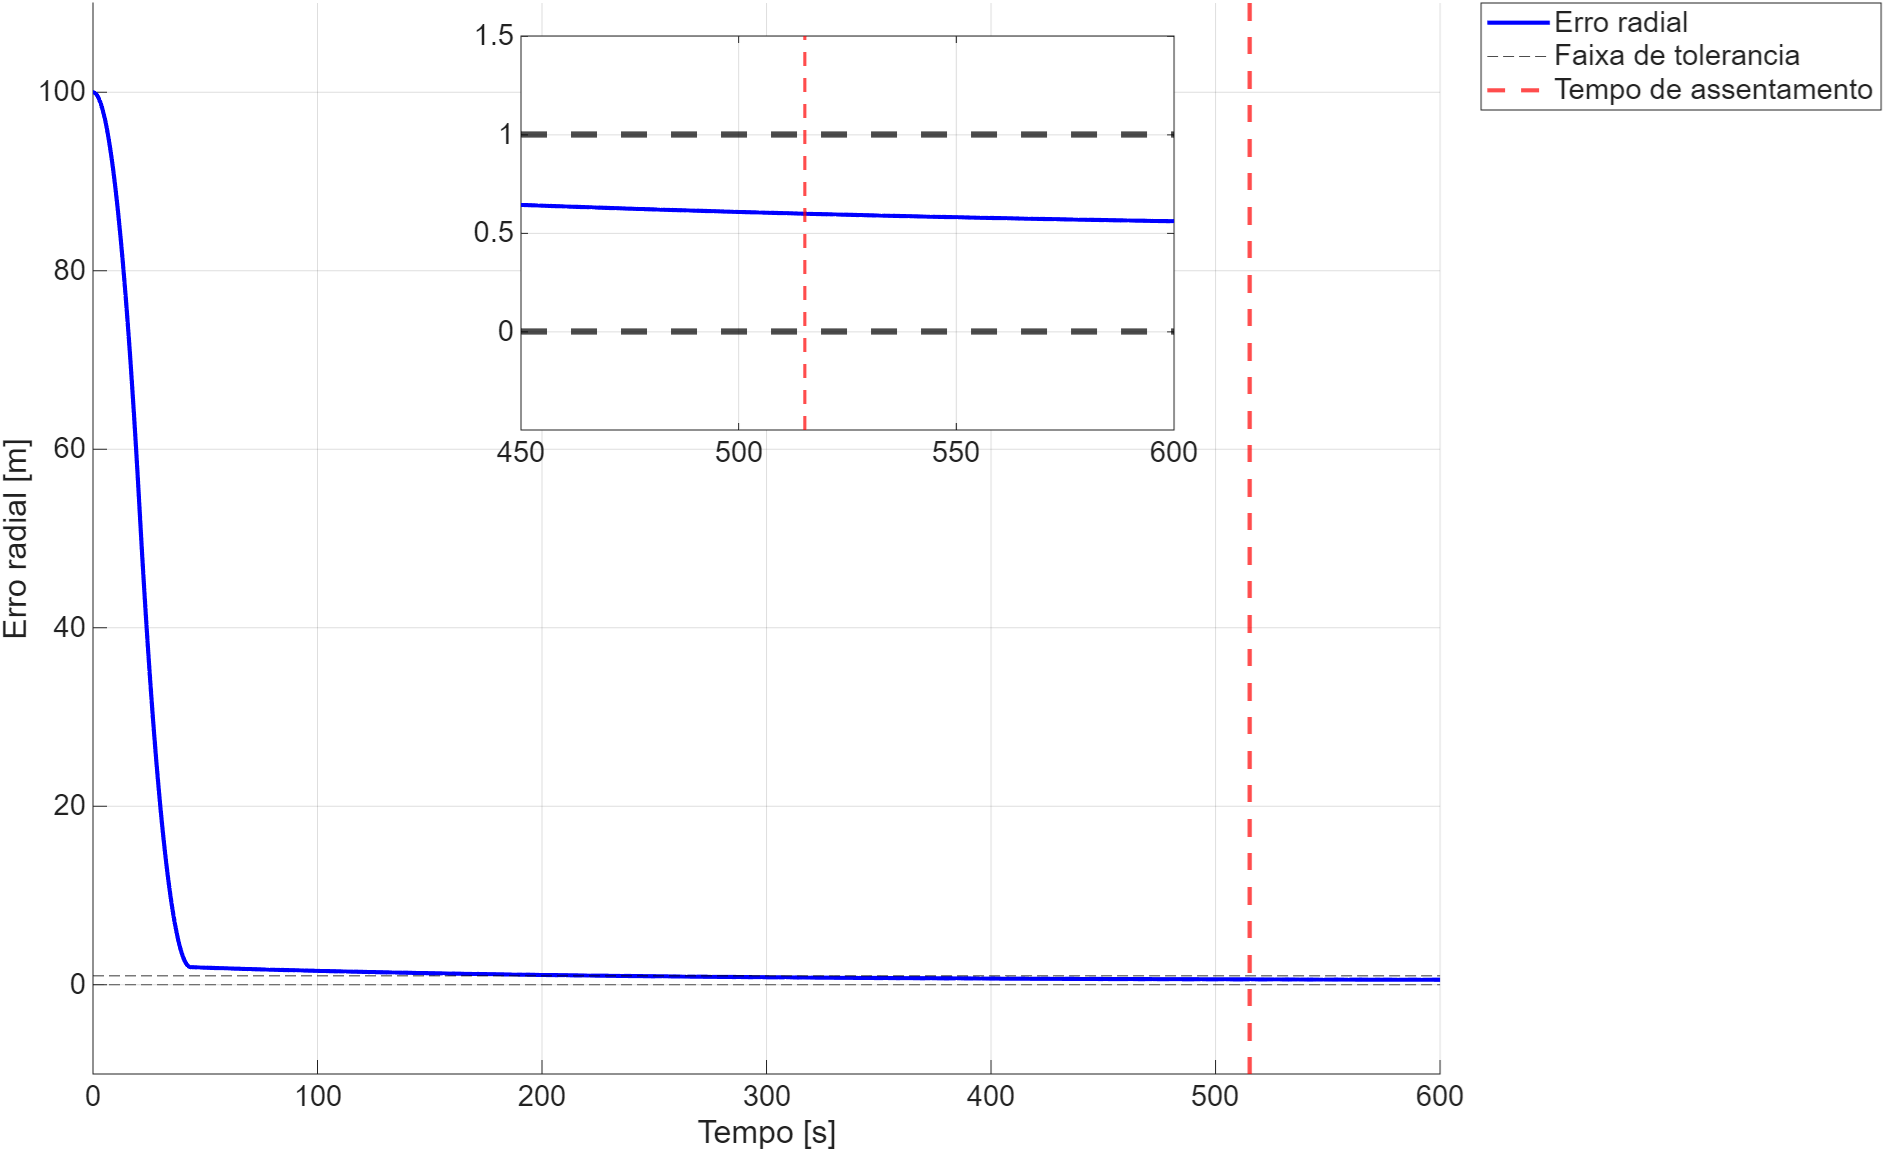
\includegraphics[width=1\linewidth]{4 Resultados e discussoes/Imagens/2 App curta distancia/6a Erro radial.png}
\caption{Erro radial no referencial \gls{lvlh}.}
\label{fig:cap4_erro_radial}
\end{figure}

De forma análoga{,} a Figura~\ref{fig:cap4_erro_alongtrack} mostra a evolução do erro de posição na componente along-track. Observa-se o decaimento do erro em direção ao valor final prescrito e{,} novamente{,} a identificação do instante em que o perseguidor é considerado estabilizado segundo o mesmo critério de tolerância.

\begin{figure}[H]
\centering

\includegraphics[width=1\linewidth]{4 Resultados e discussoes/Imagens/2 App curta distancia/6b Erro alongtrack.png}
\caption{Erro along-track no referencial \gls{lvlh}.}
\label{fig:cap4_erro_alongtrack}
\end{figure}

A Figura~\ref{fig:cap4_erro_crosstrack} apresenta o erro de posição na componente cross-track. Nesse caso{,} o erro permanece dentro da faixa de tolerância desde o início da aproximação de curta distância{,} o que se reflete no tempo de assentamento nulo reportado na Tabela~\ref{tab:cap4_app_curta_tempos_assentamento}.

\begin{figure}[H]
\centering
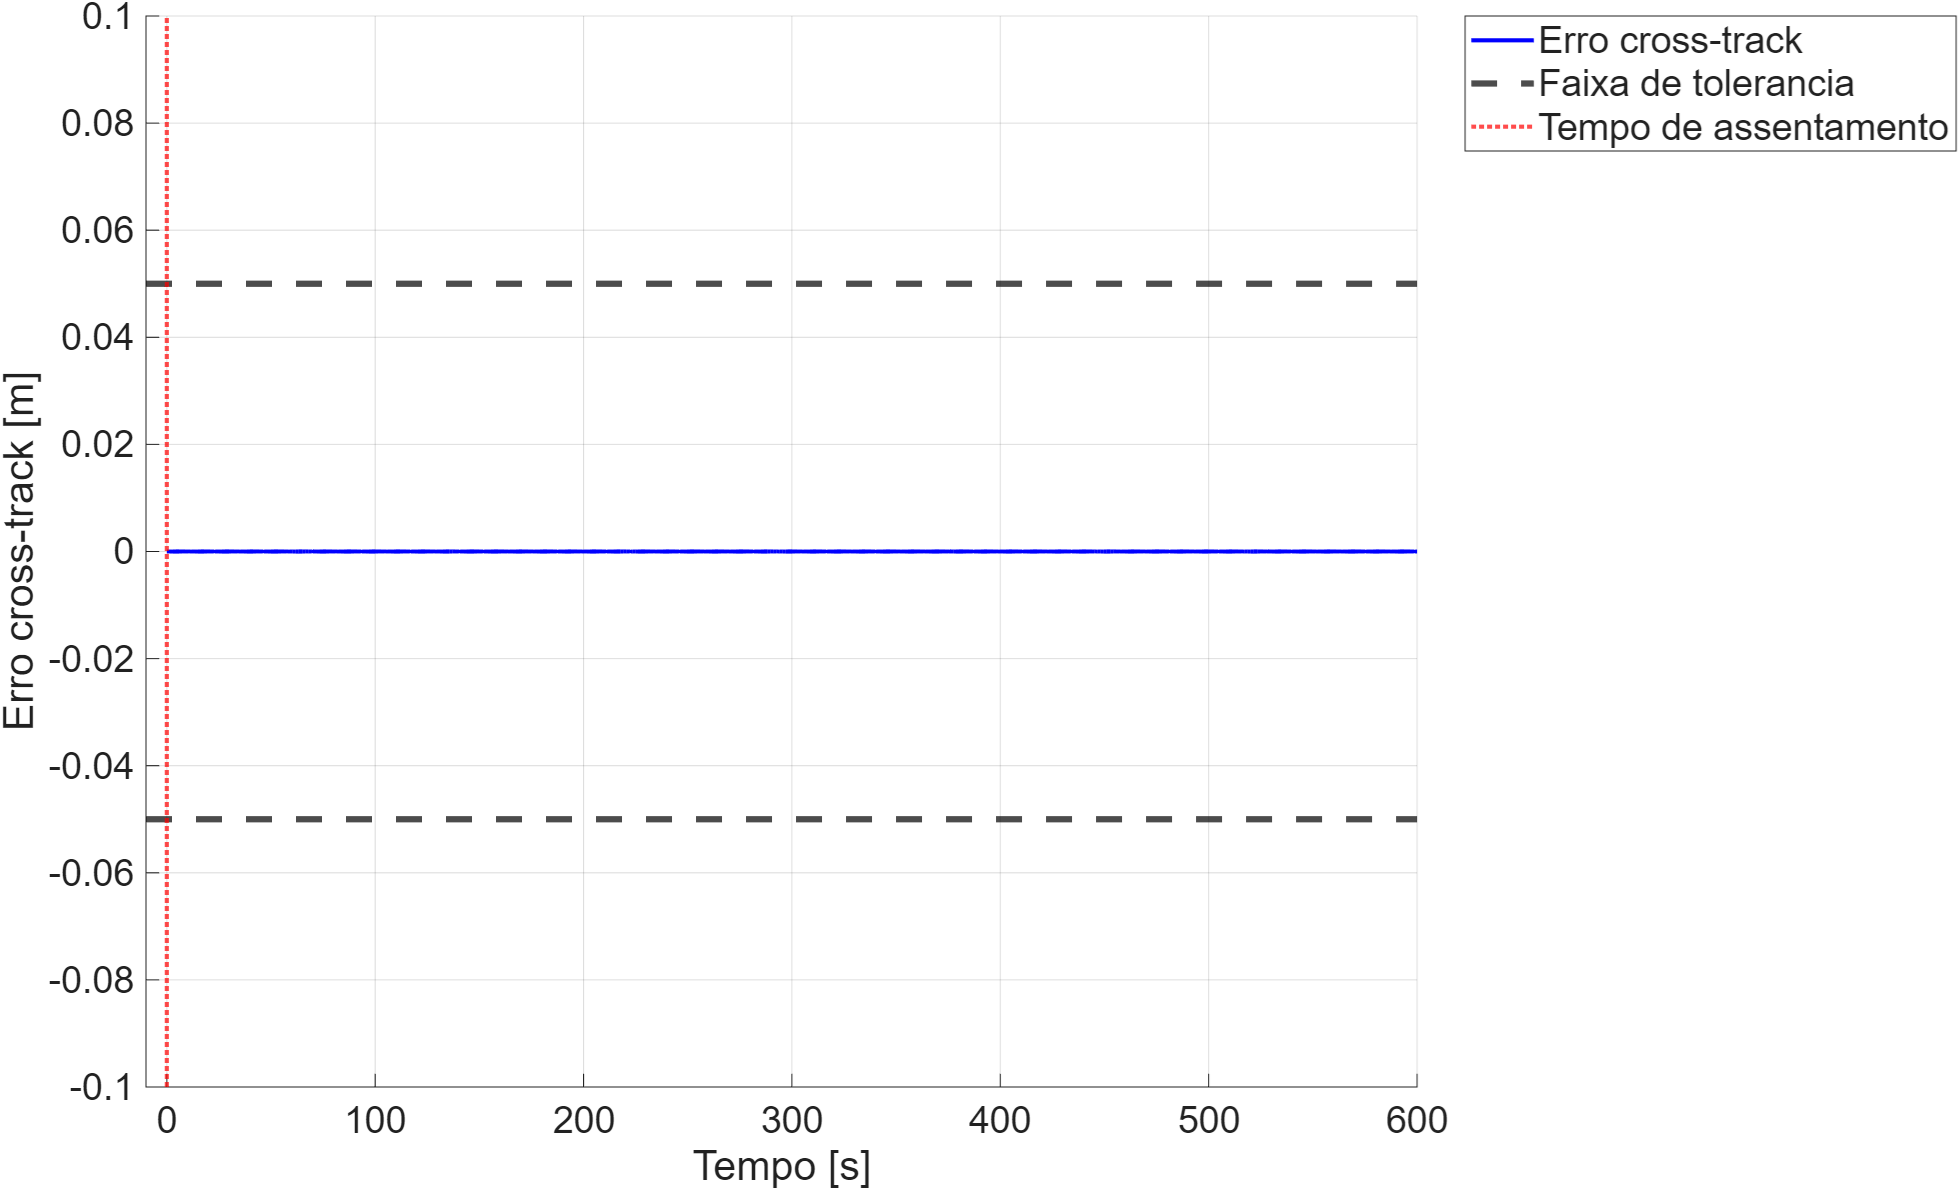
\includegraphics[width=1\linewidth]{4 Resultados e discussoes/Imagens/2 App curta distancia/6c Erro crosstrack.png}
\caption{Erro cross-track no referencial \gls{lvlh}.}
\label{fig:cap4_erro_crosstrack}
\end{figure}


\subsection{Picos de posição{,} velocidade e aceleração de controle}

A Tabela~\ref{tab:cap4_app_curta_picos_pos_vel} resume os picos absolutos de posição e de velocidade relativa por componente LVLH{,} destacando que a dinâmica permanece contida dentro dos limites impostos pela própria configuração inicial.
\begin{table}[H]
\centering
\caption{Picos absolutos de posição e velocidade relativa em LVLH.}
\label{tab:cap4_app_curta_picos_pos_vel}
\begin{tabularx}{\linewidth}{|
  >{\raggedright\arraybackslash}X|
  >{\raggedright\arraybackslash}X|
  >{\raggedleft\arraybackslash}X|
  >{\centering\arraybackslash}X|}
\hline
\multicolumn{1}{|c|}{\textbf{Grandeza}} &
\multicolumn{1}{c|}{\textbf{Componente}} &
\multicolumn{1}{c|}{\textbf{Valor máximo absoluto}} &
\multicolumn{1}{c|}{\textbf{Unidade}} \\
\hhline{|=|=|=|=|}
Posição relativa   & Along-track & $353{,}777$   & m   \\
\hline
Posição relativa   & Cross-track & $0{,}000$     & m   \\
\hline
Posição relativa   & Radial      & $100{,}009$   & m   \\
\hline
Velocidade relativa & Along-track & $0{,}300000$ & m/s \\
\hline
Velocidade relativa & Cross-track & $0{,}000000$ & m/s \\
\hline
Velocidade relativa & Radial      & $0{,}300000$ & m/s \\
\hline
\end{tabularx}
\end{table}

O esforço de controle proporcional-derivativo aplicado na aproximação curta é caracterizado pelos picos de aceleração de comando e pelos limites de velocidade relativa impostos pelo regulador. A Tabela~\ref{tab:cap4_app_curta_controle_pd} apresenta os picos de aceleração por componente \gls{lvlh} e os limites máximos de velocidade relativa utilizados na simulação.

\begin{table}[H]
\centering
\caption{Picos de aceleração de controle e limites de velocidade relativa.}
\label{tab:cap4_app_curta_controle_pd}
\begin{tabularx}{\linewidth}{|
  >{\raggedright\arraybackslash}X|
  >{\raggedright\arraybackslash}X|
  >{\raggedleft\arraybackslash}X|
  >{\centering\arraybackslash}X|}
\hline
\multicolumn{1}{|c|}{\textbf{Grandeza}} &
\multicolumn{1}{c|}{\textbf{Componente}} &
\multicolumn{1}{c|}{\textbf{Valor máximo absoluto}} &
\multicolumn{1}{c|}{\textbf{Unidade}} \\
\hhline{|=|=|=|=|}
Aceleração de controle PD & Radial      & $1{,}000000$ & m/s$^{2}$ \\
\hline
Aceleração de controle PD & Along-track & $1{,}000000$ & m/s$^{2}$ \\
\hline
Aceleração de controle PD & Cross-track & $0{,}000000$ & m/s$^{2}$ \\
\hline
Limite de velocidade relativa & Radial      & $0{,}300000$ & m/s \\
\hline
Limite de velocidade relativa & Along-track & $0{,}300000$ & m/s \\
\hline
Limite de velocidade relativa & Cross-track & $0{,}030000$ & m/s \\
\hline
\end{tabularx}
\end{table}

A Figura~\ref{fig:cap4_acel_controle} apresenta a aceleração de controle exercida pelo controlador \gls{pd} nos três eixos do referencial \gls{lvlh} do perseguidor{,} responsável pela translação nesta fase de aproximação de curta distância. Nota-se que a aceleração permanece dentro dos limites estabelecidos de $\pm 1$ m/s$^{2}$ e tende rapidamente a zero após o regime transitório{,} indicando que o controlador deixa de atuar de forma significativa quando a estabilização é alcançada.

\begin{figure}[H]
\centering

\includegraphics[width=1\linewidth]{4 Resultados e discussoes/Imagens/2 App curta distancia/7 Aceleracao controle.png}
\caption{Aceleração de controle.}
\label{fig:cap4_acel_controle}
\end{figure}


\subsection{Efeito da saturação de velocidade relativa}

Por fim{,} a Tabela~\ref{tab:cap4_app_curta_vel_raw} compara os picos de velocidade relativa que seriam obtidos sem limitação (velocidades provenientes diretamente do modelo de Hill/Clohessy--Wiltshire) com os limites efetivamente impostos pelo regulador de velocidade. Observa-se que{,} sem saturação{,} as velocidades poderiam atingir alguns metros por segundo nas componentes along-track e radial{,} ao passo que o controlador restringe a dinâmica a $0{,}3$ m/s na região distante e a $0{,}03$ m/s na vizinhança do alvo.

\begin{table}[H]
\centering
\caption{Comparação entre picos de velocidade relativa não saturada e limites impostos.}
\label{tab:cap4_app_curta_vel_raw}
\begin{tabularx}{\linewidth}{|
  >{\raggedright\arraybackslash}X|
  >{\raggedright\arraybackslash}X|
  >{\raggedleft\arraybackslash}X|
  >{\raggedleft\arraybackslash}X|}
\hline
\textbf{Grandeza} &
\textbf{Componente} &
\textbf{Valor máximo absoluto} &
\textbf{Unidade} \\
\hhline{|=|=|=|=|}
Velocidade relativa não saturada & Radial & $4{,}514556$ & m/s \\
\hline
Velocidade relativa não saturada & Along-track & $8{,}620118$ & m/s \\
\hline
Velocidade relativa não saturada & Cross-track & $0{,}000000$ & m/s \\
\hline
Limite de velocidade relativa & Radial & $0{,}300000$ & m/s \\
\hline
Limite de velocidade relativa & Along-track & $0{,}300000$ & m/s \\
\hline
Limite de velocidade relativa & Cross-track & $0{{,}}030000$ & m/s \\
\hline
\end{tabularx}
\end{table}

Com o objetivo de tornar a translação do perseguidor suave{,} adotou-se saturação de aceleração de até $\pm 1$ m/s$^{2}$. A Figura~\ref{fig:cap4_acel_saturada} apresenta as medições dessa aceleração saturada ao longo do tempo.

\begin{figure}[H]
\centering
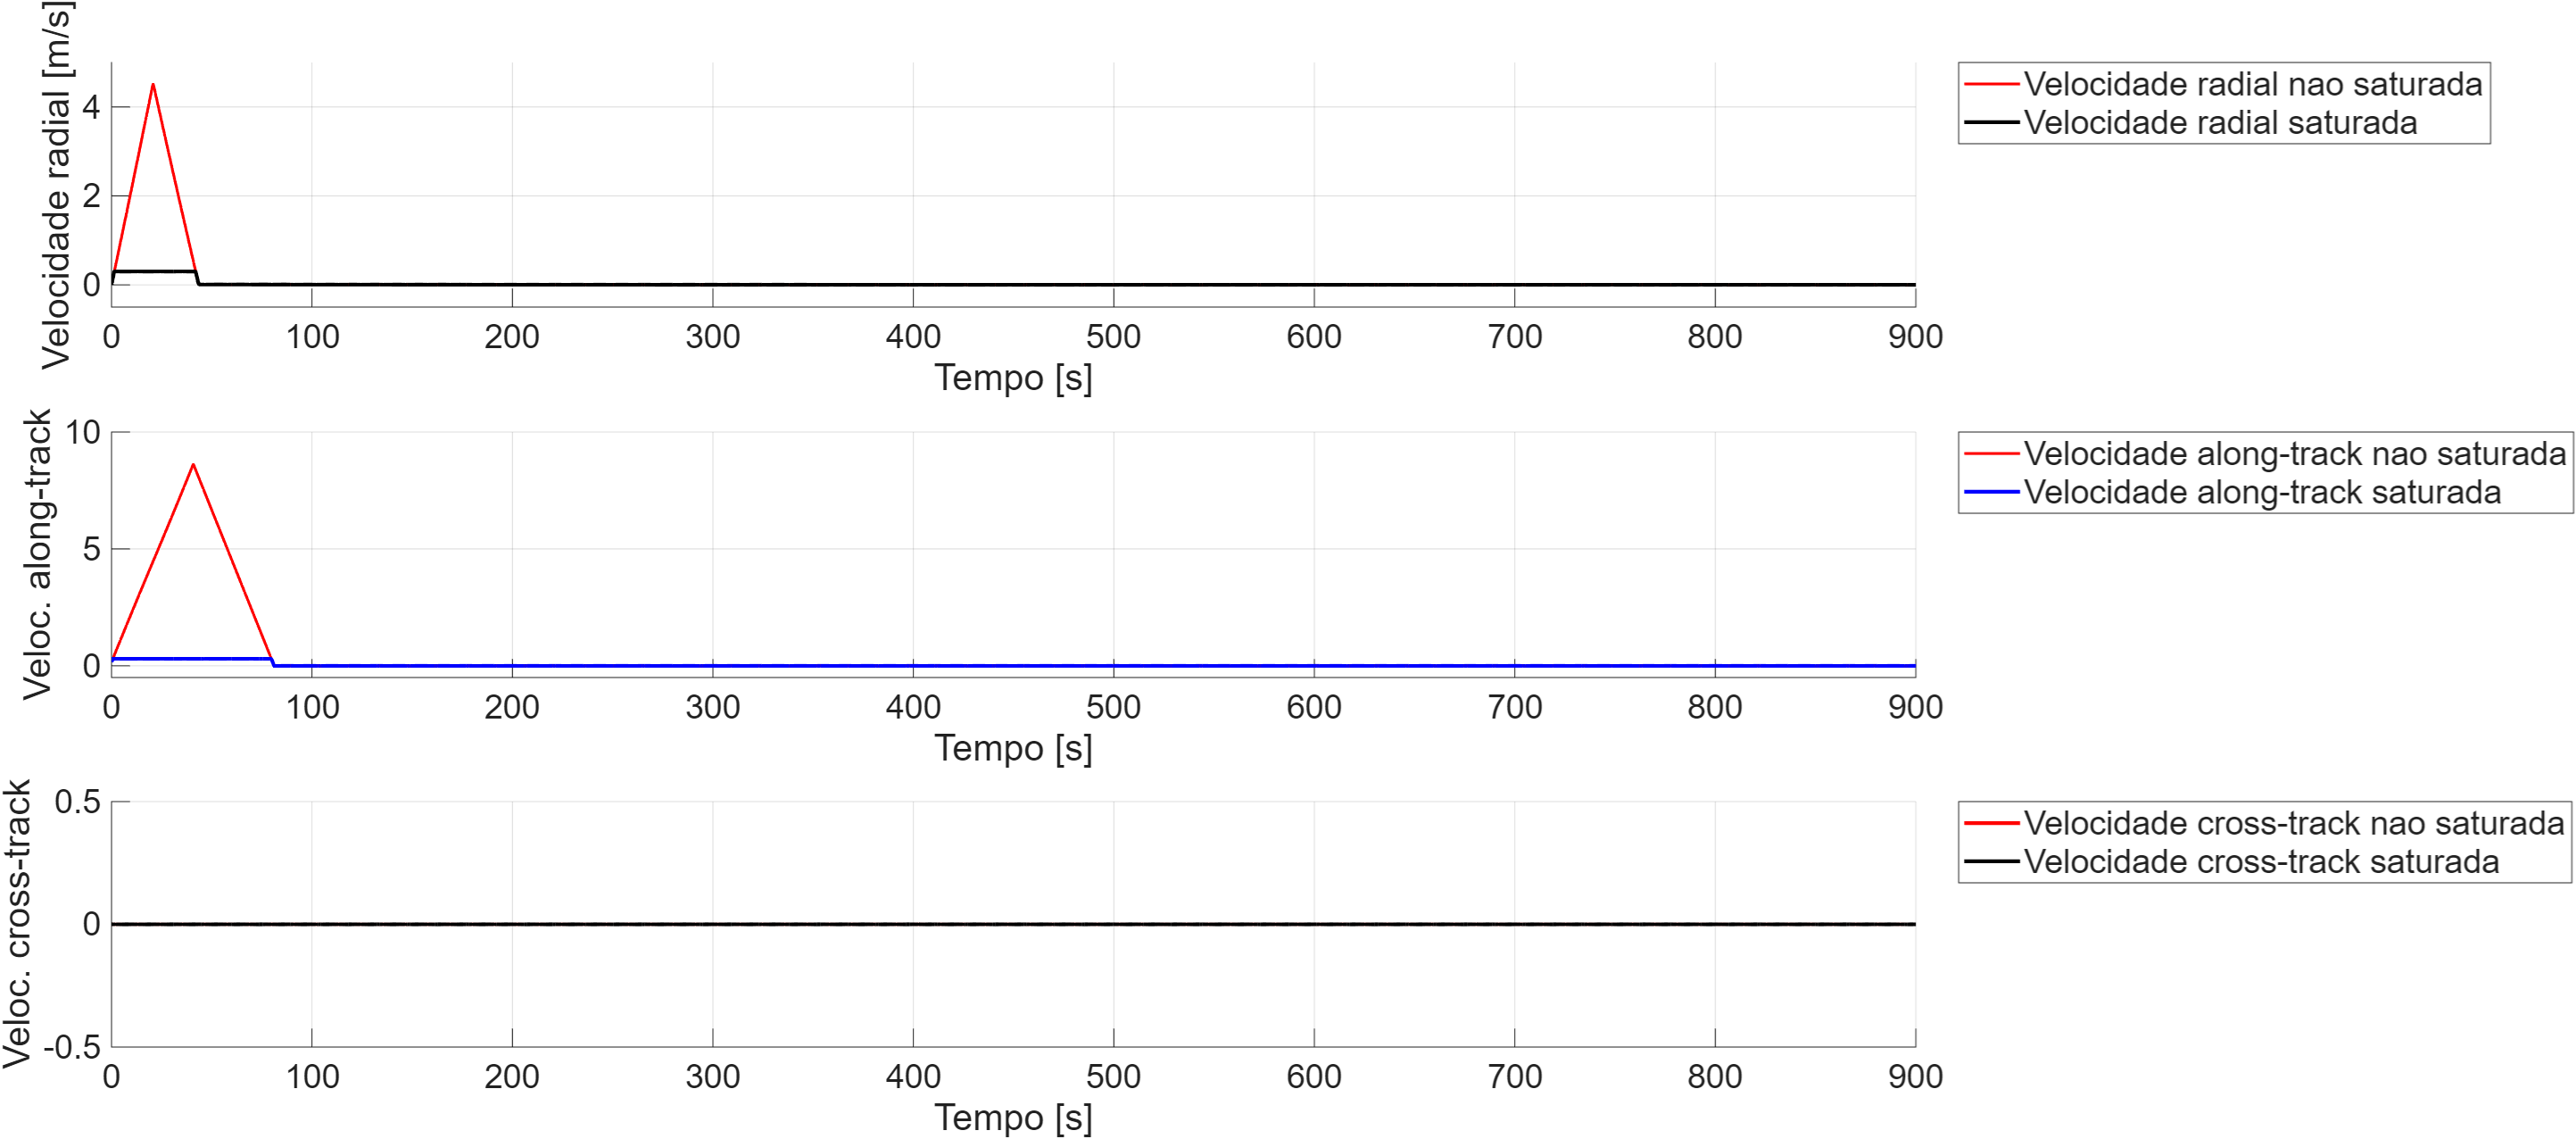
\includegraphics[width=1\linewidth]{4 Resultados e discussoes/Imagens/2 App curta distancia/8 Veloc saturada.png}
\caption{Aceleração de controle.}
\label{fig:cap4_acel_saturada}
\end{figure}